%%%%%%%%%%%%%%%%%%%%%%%%%%%%%%%%%%%%%%%%%%%%%%%%%%%%%%%%%%%%
%
% Authors:       Nina Wiedemann, Benjamin Ummenhofer, Diana Wofk, 
%                Quentin Leboutet, and Michael Paulitsch
%
% Description:   The SYCL of Life: Evolutionary Kernel Optimization 
%                with Large Language Models
%
% Section:       Appendix
%
%%%%%%%%%%%%%%%%%%%%%%%%%%%%%%%%%%%%%%%%%%%%%%%%%%%%%%%%%%%%
\newpage
\appendix
\FloatBarrier
\section{Summary of the Related Works} \label{app:relatedwork}
\begin{table*}[ht]
	\centering
	\caption{Overview of related work on LLM-based kernel generation and optimization. Methods are 
		grouped by approach: benchmarks, prompting-validation loops, multi-agent, and finetuning. Hardware is 
		GPU unless denoted otherwise.}
	\label{tab:related_work}
	\resizebox{\textwidth}{!}{%
		\begin{tabular}{llllll}
			\toprule
			\textbf{Reference} & \textbf{Language} & \textbf{Hardware} & \textbf{Benchmark [Count]} & \textbf{Method} & \textbf{Key Features} \\
			\midrule
			\multicolumn{6}{c}{\textit{Benchmarks}} \\
			\midrule
			KernelBench~\citep{ouyang2025kernelbench} & CUDA / Triton & NVIDIA & KernelBench [250] & Repeated prompting & De-facto standard \\
			MultiKernelBench~\citep{wen2025multikernelbench} & CUDA / Pallas / AscendC & NVIDIA / TPU / NPU & KernelBench revised [285] & Prompting & Multi-platform \\
			TritonBench~\citep{li2025tritonbench} & Triton & NVIDIA & TritonBench [184] & Prompting & Triton-specific \\
			NPUEval~\citep{kalade2025npueval} & C++ AIE & AMD NPU & Custom [102] & Prompting + RAG & NPU focus \\
			\midrule
			\multicolumn{6}{c}{\textit{Approaches based on inference-validation loops}} \\
			\midrule
			Robust-kbench~\citep{lange2025towards} & CUDA & NVIDIA & KernelBench + Custom [269] & Evolve & Robustness focus \\
			cuPilot~\citep{chen2025cupilot} & CUDA & NVIDIA & KernelBench L1 [100] & Evolve & Strategy coordination \\
			KernelFalcon~\citep{kernelfalcon} & Triton & NVIDIA & KernelBench [250] & Repeated prompting & 100\% correctness \\
			Opal~\citep{zaeed2025opal} & CUDA / HIP & NVIDIA / AMD & Custom [8] & Prompting + 3 profilers & Modular profiling \\
			SwizzlePerf~\citep{tschand2025swizzleperf} & HIP & AMD & Custom [10] & HW-aware prompting & Microarch knowledge \\
			TritonForge~\citep{li2025tritonforge} & Triton & NVIDIA & TritonBench [185] & Profiling-guided & Automated profiling \\
			KernelEvolve~\citep{liao2025kernelevolve} & Triton / CuTE & NVIDIA / AMD & KernelBench [250] & Tree search & Meta scaling \\
			Geak~\citep{wang2025geak} & Triton & AMD & TritonBench-revised & Prompting + Reflection & AI agent \\
			PEAK~\citep{tariq2025peak} & CUDA / HIP / HLSL & NVIDIA / AMD / Qualcomm & MatMul & Natural transformations & Iterative + Modular \\
			\midrule
			\multicolumn{6}{c}{\textit{Multi-Agent Approaches}} \\
			\midrule
			Astra~\citep{wei2025astra} & CUDA & NVIDIA & Custom [3] & Multi-agent & Plan/Code/Test/Profile \\
			CudaForge~\citep{zhang2025cudaforge} & CUDA & NVIDIA & KernelBench [25] & Coder + Judge & Hardware feedback \\
			STARK~\citep{dong2025stark} & CUDA & NVIDIA & KernelBench [250] & Plan + Code + Debug & Strategic agents \\
			QiMeng~\citep{zhu2025qimeng} & Triton & NVIDIA & KernelBench + TritonBench & Macro/Micro coding & Two-stage thinking \\
			PRAGMA~\citep{lei2025pragma} & Triton / C++ & NVIDIA / Intel CPU & KernelBench & Coder + Verifier + Conductor & Profiling-reasoned \\
			AKG Agent~\citep{du2025akg} & Triton & NVIDIA / Ascend NPU & KernelBench L1 [100] & Coder + Designer & Cross-platform \\
			\midrule
			\multicolumn{6}{c}{\textit{Finetuning Approaches}} \\
			\midrule
			Kevin~\citep{baronio2025kevin} & CUDA & NVIDIA & KernelBench [100] & Multi-turn RL & Turn-level rewards \\
			CUDA-L1~\citep{li2025cuda} & CUDA & NVIDIA & KernelBench [250] & Contrastive RL & 3.12$\times$ speedup \\
			CUDA-L2~\citep{su2025cuda} & CUDA & NVIDIA (A100) & HGEMM [1000] & Multi-stage RL + NCU & Beats cuBLAS (+11\%) \\
			TritonRL~\citep{woo2025tritonrl} & Triton & NVIDIA & KernelBench [200] & SFT + GRPO & No reward hacking \\
			\midrule
			\textbf{KernelFoundry (Ours)} & \textbf{SYCL / CUDA / Triton} & \textbf{Intel / NVIDIA} & \textbf{KernelBench + robust-kbench} & \textbf{MAP-Elites + Meta-prompt} & \textbf{QD + Parameter optim.} \\
			\bottomrule
		\end{tabular}%
	}
\end{table*}

\section{Implementation Details} \label{app:implementation}

\subsection{System Configuration}

KernelFoundry is implemented in Python with the following core dependencies:
\begin{itemize}\itemsep0em
    \item \textbf{LLM inference}: OpenAI API, Anthropic API, vLLM for local models
    \item \textbf{Compilation}: Intel oneAPI DPC++ 2025.2, NVIDIA CUDA Toolkit 12.8, Triton 3.5
    \item \textbf{Profiling}: Profiling Tools Interfaces for GPU (unitrace 2.3) for SYCL, NVIDIA Nsight Compute 2025.3.0.0 for CUDA
    \item \textbf{Testing}: PyTorch 2.9
\end{itemize}


\subsection{Benchmarking kernel runtime}\label{app:benchmarking}

In contrast to prior work, we implement several improvements in the kernel benchmarking to reduce the variance of runtime measurements. Our implementation proceeds as follows: First, we run a fixed number of initial trials to determine the rough runtime of the kernel. This initial measurement informs the number of warmup trials and main trials, which are set based on a minimal total \textit{time} rather than a fixed amount of trials (if the kernel is slow, less warmup trials and main trials are required). Furthermore, we noticed that for very fast kernels, the \texttt{torch.cuda.synchronize} or \texttt{torch.xpu.synchronize} operation has a significant overhead. We reduce this overhead by running an inner loop within the main trials, such that multiple trials are executed before each synchronize.\\
For all experiments, we set the minimum warmup time to 1 second, the mininum warmup iterations to 10, the inner-loop minimum time to 0.01 seconds, the minimum number of main iterations to 10 and the minimum runtime of the main performance measurement to 1s. This ensures that measured durations are comfortably larger than the timer precision and synchronization overhead while guaranteeing enough measurements to compute runtime statistics.

Furthermore, we noticed that the runtime measurement of \textit{backward} operations in robust-kbench has a significant overhead due to using \texttt{torch.autograd}, rather than measuring the kernel execution time directly. We found a way to measure the isolated runtime of the kernel which is more stable. However, for the reference we still need to measure \texttt{torch.autograd.grad}. This leads to high speedups for backward operations as can be seen in \autoref{tab:robust_kbench_by_task}; however, this appeared as a minor drawback to us compared to an incorrect kernel runtime measurement.

\subsection{Profiler Feedback}

For correct kernels, optional profiling provides performance insights. We collect and provide the following information:
\begin{itemize}\itemsep0em
    \item \textbf{Execution time}: Wall-clock runtime
    \item \textbf{Memory bandwidth}: Achieved vs.\ theoretical peak (via \texttt{unitrace} or Nsight Compute)
    \item \textbf{Compute utilization}: ALU occupancy, instruction throughput
    \item \textbf{Bottleneck identification}: Memory-bound vs.\ compute-bound classification
\end{itemize}

Profiler feedback is structured into natural language summaries (e.g., ``Kernel is memory-bound 
at 45\% of peak bandwidth. Consider shared memory tiling to improve data reuse.'').


\subsection{Hyperparameters}\label{app:hyperparameters}

Table~\ref{tab:hyperparameters} lists the default hyperparameters used in our experiments. 
The number of iterations depends on the experiment: For our experiment on SYCL kernel generation and comparison to OpenEvolve, we use 40 iterations with 8 generations each. This is aligned with Robust-kbench~\cite{lange2025towards} who also sample 8 suggestions from the LLM in each iteration and show the results over 40 iterations. For a fair comparison to The AI CUDA Engineer~\cite{lange2025ai}, we set the number of iterations to 40 and the population size to 4 to align with their experimental setup.\\ As explained in \autoref{sec:experiments}, we also align the LLMs to the ones in the baseline papers. For the SYCL experiment, we chose to prompt a powerful language model (Claude Sonnet~4.5) in the first iteration to avoid getting trapped in a local minimum at the beginning. After the first iteration, we use an ensemble of GPT~5~mini and GPT~4.1 (equal weights). After the 40 iterations, we run 2 iterations of parameter optimization. 

\begin{table}[ht]
\centering
\begin{tabular}{lc}
\toprule
\textbf{Parameter} & \textbf{Value} \\
\midrule
\multicolumn{2}{l}{\textit{Evolution}} \\
Max generations & 40 (*) \\
Population per generation & 8 (*) \\
Selection strategy & Curiosity-driven \\
Archive dimensions & 4 \\
Bins per dimension & 4 \\
\midrule
\multicolumn{2}{l}{\textit{Evaluation}} \\
Warmup iterations & 10 \\
Timing iterations & 100 \\
% Correctness tolerance (relative) & $10^{-5}$ \\
% Correctness tolerance (absolute) & $10^{-8}$ \\
Target speedup & 2.0$\times$ \\
\midrule
\multicolumn{2}{l}{\textit{Meta-prompting}} \\
Prompt update frequency & Every 10 generations \\
Max prompt mutations & 3 per update \\
Prompt archive size & 16 \\
\midrule
\multicolumn{2}{l}{\textit{LLM}} \\
Temperature & 0.3 \\
Max tokens & 8000 \\
Top-p & 1 \\
\bottomrule
\end{tabular}
\caption{Hyperparameters for KernelFoundry. (*) number of operations, population size, and LLM model vary dependent on the experiment.}
\label{tab:hyperparameters}
\end{table}


\section{Distributed System \& Custom Task Input}\label{app:custom_task_infrastructure}

\mypara{Infrastructure} As shown in \autoref{fig:infrastructure}, the KernelFoundry pipeline utilizes a lightweight main thread that interacts with four servers. The server processes can run on a single machine or on multiple remote machines in the same network. 
\begin{enumerate}\itemsep0em
    \item \textbf{LLM Server}: Hosts the generation model (Cloud services with REST-API or local vLLM instances).
    \item \textbf{Compilation Workers}: Executes compiler toolchains (DPC++, nvcc). Does not need a GPU.
    \item \textbf{Execution Workers}: Run correctness tests and benchmarks on GPU nodes. Connected via a task queue ensuring single-task-per-GPU isolation.
    \item \textbf{Database Server}: Stores all generated kernels, evaluation results, and evolutionary state for reproducibility and analysis.
\end{enumerate}
The LLM server, compile worker, and execution worker are connected via a load balancer and queue system and allows to scale the number of workers and increase parallelism.

\mypara{Custom task} Tasks are defined by a set of files with special markers, making them highly customizable and easy to integrate into existing projects.
A task is defined by a config file in YAML format containing hyperparameters; a python module with a build function and correctness and performance tests defined in the pytest framework; and a language specific file for the generated code.
Special markers are used to define sections for the reference code, optional user instructions, and optional initial kernel implementations passed to the model. 

\begin{figure}[t]
    \centering
    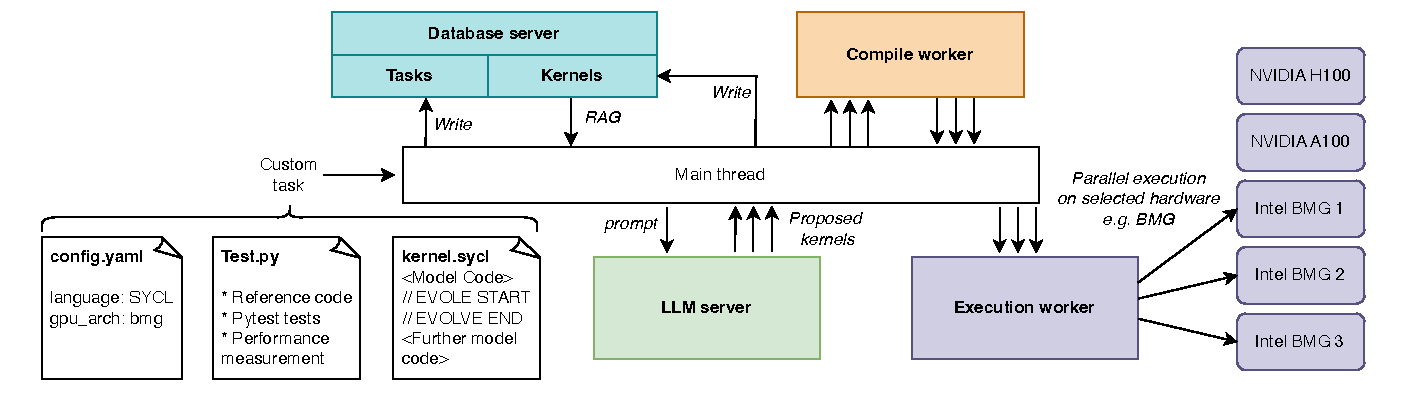
\includegraphics[width=\textwidth]{Figures/custom_input_infrastructure.pdf}
    \caption{Overview of the KernelFoundry infrastructure and the custom task format}
    \label{fig:infrastructure}
\end{figure}

\section{KernelBench task filtering}\label{app:kernelbench_filtering}

We follow~\citet{lange2025towards} and~\citet{metr} and filter out KernelBench tasks that are flawed. \citet{lange2025towards} propose 5 criteria: (1) small output value range, (2) small output StD, (3) small output StD across any axis, (4) small impact of inputs on the output, (5) baseline inefficiencies. For our experiments, we select the same task set as \cite{lange2025towards} to ensure full consistency. 

However, it is worth noting that we generally believe that criterion (3) is too strict, as we did not observe issues with the kernels generated for such tasks, and e.g. for outputs with shape 2 along one axis the StD can naturally be low. Tasks with baseline inefficiencies (5) do not necessarily need to be removed either, as the comparison is still fair. \citet{lange2025towards} used an LLM to identify these tasks which sometimes gave wrong responses on closer inspection. Filtering according to criteria (1), (2) and (4) would retain 223 tasks across level 1, 2 and 3.

The set of representative tasks (20 L1, 20 L2, see Section~\ref{sec:experimental_benchmarks}) was selected based on the following criteria:
\begin{enumerate}\itemsep-0.3em
    \item Diversity: 20 tasks from level 1, 20 from level 2, covering all kind of operations (matmul, conv, conv transpose, activation functions, etc.)
    \item Uncompromised: We only select tasks that comply with criteria (1)-(5)  by \citet{lange2025towards}, i.e. tasks that are not listed as ``compromised tasks'' in \cite{lange2025towards} Appendix A.2 and A.3.
    \item Availability of correct baseline kernels: For a fair comparison to \cite{lange2025ai}, we select only tasks for which they publish a kernel as part of their Huggingface dataset, and filtering only for the ones where their fastest kernel (per task) passes our correctness tests. Since our tests are more strict than the test used in \cite{lange2025ai}, 53 out of the 229 kernels failed our tests.
\end{enumerate}

\section{Prompts}\label{app:prompts}

\subsection{Main prompt}

\begin{promptbox}
You are a $<$language$>$ programming expert specializing in GPU kernel optimization. Given a reference $<$reference-language$>$ implementation, your objective is to create a performant  kernel with identical functionality. The code you generate will be pasted into an existing project. Make sure to follow the existing code structure and function signatures. The $<$language$>$ code you generate will be saved in $<$ kernel.cpp / kernel.cu $>$ and loaded using \texttt{torch.utils.cpp\_extension.load()}:
\begin{verbatim}
```load(name=task_name, sources=[<kernel.cpp / kernel.cu>]```
\end{verbatim}
Later, the function will be called via \texttt{load(name=task\_name, ...).forward} and thoroughly tested.


\textbf{Examples:}\\
Here is an example of a correct $<$language$>$ kernel for a given $<$reference-language$>$ reference:\\
$<$example-reference-code$>$\\
$<$example-kernel-code$>$

\vspace{0.5em}

\textbf{Reference code / Task:}\\
This is the reference $<$reference-language$>$ implementation:\\
$<$reference-code$>$

\vspace{0.5em}

\textbf{Top performing kernel:}\\
This is the best  kernel tested so far (Runtime: $<$top-kernel-runtime$>$):\\
$<$top-kernel-code$>$

\vspace{0.5em}

\textbf{Last tested kernel:}\\
Here is the last  kernel we tested (Runtime: $<$last-kernel-runtime$>$):\\
$<$last-kernel-code$>$\\
Console output from running this kernel:\\
$<$last-kernel-log$>$

\vspace{0.5em}

\textbf{Hardware specification:}\\
Your code will run on the following hardware:\\
$<$hardware-specs$>$\\
Please consider the hardware specifications when improving the code. 

\vspace{0.5em}

\textbf{Main Instructions:}
\vspace{-0.5em}
\begin{enumerate}\itemsep-0.5em
    \item Provide a functional kernel that matches the reference implementation.
    \item Use constructs to efficiently run the code on GPU.
    \item Provide the complete code in a code block.
\end{enumerate}

\textbf{Optimization strategies:}\\
$<$evolvable-optimization-strategies$>$

\vspace{0.5em}
    
\textbf{Critical Requirements:}
\vspace{-0.5em}
\begin{enumerate}\itemsep-0.3em
    \item The kernel must exactly match the reference's functionality.
    \item The code must compile and run properly on the GPU.
    \item Do not cache or reuse previous results; ensure the code executes fully on each run.
\end{enumerate}

\textbf{Response Format:}\\
Please structure your response as follows:
\vspace{-0.5em}
\begin{enumerate}\itemsep-0.3em
    \item Analysis: Summarize the issues found in the previous kernel and log. Explain your proposed changes and optimizations.
    \item Code: Provide the complete, improved $<$language$>$ code in code blocks:
\end{enumerate}
\vspace{-1em}
\begin{verbatim}
```
Your code here
```
\end{verbatim}
\end{promptbox}



\subsection{Templated kernels for parameter optimization}\label{app:templated_prompt}

To guide the model towards converting parameters to template parameters which can then be tuned with our pipeline, we use the following prompt and code example: 

\begin{promptbox}
You are a $<$language$>$ programming expert specializing in GPU kernel optimization. Your task is to optimize a given $<$language$>$ kernel.

\textbf{Given kernel:}

Here is the $<$language$>$ kernel that we tested:

$<$Code of best generated kernel$>$

To optimize this kernel for specific hardware, please propose a templated kernel with some template parameters that can be tuned. To do so, you need to write an extension for PyTorch that implements a templated $<$language$>$ kernel and a forward function for dispatching. Select suitable parameter options by adding them as dispatch-options in the forward function.\\

\textbf{Requirements:}
\begin{itemize}
    \item The kernel should be templated on suitable parameters, e.g., block size, etc.
    \item The \texttt{forward\_templated} function should launch the kernel with the given parameter values.
    \item The \texttt{forward} function should have standard arguments corresponding to the template parameters of \texttt{forward\_templated}, and should select the correct instantiation based on the input values.
    \item The code must match the given kernel in functionality.
    \item The code should include a Pybind11 interface exposing \texttt{forward}.
\end{itemize}

Here is an example of a templated kernel in the correct format:
\end{promptbox}

\begin{lstlisting}[style=syclcode,caption={Example SYCL kernel with parameter dispatch}]
#include <sycl/sycl.hpp>
#include <torch/extension.h>
#include <c10/xpu/XPUStream.h>

// Kernel name struct at namespace scope
template <int BX, int BY>
struct ElementwiseMulKernel {};

template <int BLOCK_X, int BLOCK_Y>
void elementwise_mul_sycl_kernel(
    torch::Tensor A,
    torch::Tensor B,
    torch::Tensor C,
    int N,
    int M
) {
    auto a_data = A.data_ptr<float>();
    auto b_data = B.data_ptr<float>();
    auto c_data = C.data_ptr<float>();

    sycl::queue& q = c10::xpu::getCurrentXPUStream().queue();

    sycl::range<2> global_range(
        ((N + BLOCK_Y - 1) / BLOCK_Y) * BLOCK_Y,
        ((M + BLOCK_X - 1) / BLOCK_X) * BLOCK_X
    );
    sycl::range<2> local_range(BLOCK_Y, BLOCK_X);

    q.submit([&](sycl::handler& cgh) {
        cgh.parallel_for<ElementwiseMulKernel<BLOCK_X, BLOCK_Y>>(
            sycl::nd_range<2>(global_range, local_range),
            [=](sycl::nd_item<2> item) {
                int row = item.get_global_id(0);
                int col = item.get_global_id(1);
                if (row < N && col < M) {
                    int idx = row * M + col;
                    c_data[idx] = a_data[idx] * b_data[idx];
                }
            }
        );
    }).wait();
}

// 2. Templated forward function
template <int BLOCK_X, int BLOCK_Y>
torch::Tensor forward_templated(torch::Tensor A, torch::Tensor B) {
    int N = A.size(0);
    int M = A.size(1);
    auto C = torch::empty({N, M}, A.options());
    elementwise_mul_sycl_kernel<BLOCK_X, BLOCK_Y>(A, B, C, N, M);
    return C;
}

// 3. Dispatcher - must have arguments corresponding to the template parameters of forward_templated
torch::Tensor forward(torch::Tensor A, torch::Tensor B, int block_x, int block_y) {
    TORCH_CHECK(A.scalar_type() == torch::kFloat, "Only float32 supported in this example");
    TORCH_CHECK(A.dim() == 2 && B.dim() == 2, "Only 2D tensors supported");
    TORCH_CHECK(A.sizes() == B.sizes(), "Input sizes must match");

    if (block_x == 16 && block_y == 16) {
        return forward_templated<16, 16>(A, B);
    } else if (block_x == 32 && block_y == 8) {
        return forward_templated<32, 8>(A, B);
    } else if (block_x == 8 && block_y == 32) {
        return forward_templated<8, 32>(A, B);
    } else {
        TORCH_CHECK(false, "Unsupported block size combination");
    }
}

// 4. Pybind11 interface
PYBIND11_MODULE(TORCH_EXTENSION_NAME, m) {
    m.def("forward", &forward, "Elementwise multiplication with block size dispatch");
}
\end{lstlisting}


\section{Per-task results}\label{app:pertaskresults}

\subsection{Robust-kbench comparison}\label{robustkbench}

\begin{table*}[ht]
    \centering
    \resizebox{0.8\textwidth}{!}{
    \begin{tabular}{lrrrr}
    \toprule
     & Robust-kbench original & Robust-kbench re-evaluated & Ours & Ours + parameter optim. \\
    Operation &  &  &  &  \\
    \midrule
    layernorm\_forward & 165.678 & 55.116 & 55.625 & 55.625 \\
    llama\_ffw & 1.011 & 1.010 & 1.014 & 1.012 \\
    llama\_rmsnorm\_forward & 3.920 & 2.911 & 3.529 & 3.517 \\
    mnist\_conv\_relu\_pool\_forward & 2.790 & 3.947 & 5.068 & 5.007 \\
    mnist\_cross\_entropy\_backward & 0.958 & 10.388 & 23.905 & 23.905 \\
    mnist\_cross\_entropy\_forward & 1.933 & 0.400 & 1.434 & 1.389 \\
    mnist\_linear\_backward & 1.200 & 9.700 & 22.000 & 22.000 \\
    mnist\_linear\_forward & 2.517 & 1.558 & 1.669 & 1.520 \\
    mnist\_linear\_relu\_backward & 1.226 & 15.446 & 22.233 & 22.233 \\
    mnist\_linear\_relu\_forward & 2.494 & 1.345 & 2.726 & 2.675 \\
    mnist\_pool\_backward & 1.116 & 3.354 & 4.761 & 4.761 \\
    resnet\_block & 2.625 & 1.205 & 1.325 & 1.328 \\
    \midrule
    Average & 15.622 & 8.865 & 12.107 & 12.081 \\
    \bottomrule
    \end{tabular}
    }
\caption{Comparison on robust-kbench by task}
\label{tab:robust_kbench_by_task}
\end{table*}


\FloatBarrier

\subsection{Comparison to AI CUDA Engineer}\label{app:aicudaengineer}

\begin{table*}[b!ht]
    \centering
    \resizebox{\textwidth}{!}{
\begin{tabular}{lrrrrr}
\toprule
 & Level & AI CUDA Engineer original & AI CUDA Engineer re-evaluated & Ours & Ours + parameter optim. \\
Operation &  &  &  &  &  \\
\midrule
20\_LeakyReLU & 1 & 1.134 & 0.621 & 0.910 & 0.955 \\
21\_Sigmoid & 1 & 1.109 & 0.554 & 0.805 & 0.805 \\
25\_Swish & 1 & 1.562 & 1.016 & 1.349 & 1.402 \\
30\_Softsign & 1 & 2.474 & 1.724 & 2.895 & 2.895 \\
33\_BatchNorm & 1 & 0.619 & 0.975 & 1.017 & 1.017 \\
44\_Average\_Pooling\_1D & 1 & 1.238 & 0.643 & 0.769 & 0.824 \\
48\_Mean\_reduction\_over\_a\_dimension & 1 & 1.760 & 0.567 & 0.887 & 0.887 \\
4\_Matrix\_vector\_multiplication\_ & 1 & 0.939 & 0.897 & 0.985 & 0.990 \\
53\_Min\_reduction\_over\_a\_dimension & 1 & 2.187 & 0.981 & 1.317 & 1.317 \\
5\_Matrix\_scalar\_multiplication & 1 & 0.999 & 0.999 & 1.003 & 1.008 \\
64\_conv\_transposed\_1D & 1 & 1.021 & 0.578 & 1.017 & 1.213 \\
67\_conv\_standard\_1D & 1 & 1.411 & 1.199 & 1.566 & 1.576 \\
72\_ConvTranspose3d\_BatchNorm\_AvgPool\_AvgPool & 1 & 1.047 & 1.030 & 0.315 & 0.319 \\
76\_conv\_standard\_1D\_dilated\_strided\_\_ & 1 & 1.883 & 1.209 & 1.325 & 1.325 \\
7\_Matmul\_with\_small\_K\_dimension\_ & 1 & 0.670 & 0.612 & 1.095 & 1.135 \\
82\_conv\_depthwise\_2D\_square\_input\_square\_kernel & 1 & 1.239 & 1.530 & 0.794 & 0.794 \\
86\_conv\_depthwise\_separable\_2D & 1 & 0.808 & 0.574 & 0.940 & 0.961 \\
87\_conv\_pointwise\_2D & 1 & 0.249 & 0.499 & 1.000 & 1.000 \\
89\_cumsum & 1 & 2.214 & 1.319 & 1.824 & 2.127 \\
99\_TripletMarginLoss & 1 & 3.873 & 2.570 & 2.278 & 2.278 \\
\midrule
Average &  & 1.422 & 1.005 & 1.204 & 1.241 \\
\midrule
16\_ConvTranspose2d\_Mish\_Add\_Hardtanh\_Scaling & 2 & 1.689 & 1.684 & 0.466 & 0.469 \\
17\_Conv2d\_InstanceNorm\_Divide & 2 & 1.786 & 2.036 & 1.920 & 2.022 \\
1\_Conv2D\_ReLU\_BiasAdd & 2 & 1.170 & 1.626 & 3.322 & 3.444 \\
21\_Conv2d\_Add\_Scale\_Sigmoid\_GroupNorm & 2 & 1.786 & 1.982 & 2.891 & 2.834 \\
24\_Conv3d\_Min\_Softmax & 2 & 1.001 & 1.026 & 1.013 & 1.013 \\
32\_Conv2d\_Scaling\_Min & 2 & 1.767 & 1.537 & 2.398 & 2.655 \\
35\_Conv2d\_Subtract\_HardSwish\_MaxPool\_Mish & 2 & 1.932 & 2.331 & 1.624 & 1.669 \\
37\_Matmul\_Swish\_Sum\_GroupNorm & 2 & 1.499 & 1.804 & 1.256 & 1.443 \\
46\_Conv2d\_Subtract\_Tanh\_Subtract\_AvgPool & 2 & 1.393 & 2.333 & 5.560 & 5.622 \\
47\_Conv3d\_Mish\_Tanh & 2 & 1.086 & 1.192 & 1.361 & 1.379 \\
50\_ConvTranspose3d\_Scaling\_AvgPool\_BiasAdd\_Scaling & 2 & 1.000 & 1.019 & 3.039 & 3.099 \\
59\_Matmul\_Swish\_Scaling & 2 & 1.911 & 0.954 & 1.412 & 1.408 \\
5\_ConvTranspose2d\_Subtract\_Tanh & 2 & 1.092 & 1.153 & 0.199 & 0.200 \\
67\_Conv2d\_GELU\_GlobalAvgPool & 2 & 1.634 & 2.000 & 1.464 & 1.526 \\
70\_Gemm\_Sigmoid\_Scaling\_ResidualAdd & 2 & 1.713 & 0.781 & 1.592 & 1.881 \\
73\_Conv2d\_BatchNorm\_Scaling & 2 & 1.024 & 0.924 & 1.739 & 1.741 \\
82\_Conv2d\_Tanh\_Scaling\_BiasAdd\_Max & 2 & 1.999 & 2.712 & 3.883 & 3.744 \\
85\_Conv2d\_GroupNorm\_Scale\_MaxPool\_Clamp & 2 & 1.241 & 1.322 & 2.037 & 2.077 \\
97\_Matmul\_BatchNorm\_BiasAdd\_Divide\_Swish & 2 & 2.277 & 1.688 & 1.662 & 1.726 \\
99\_Matmul\_GELU\_Softmax & 2 & 2.778 & 2.020 & 2.183 & 2.124 \\
\midrule
Average &  & 1.589 & 1.606 & 2.051 & 2.104 \\
\bottomrule
\end{tabular}

    }
\caption{Comparison of speedup to the AI CUDA Engineer~\cite{lange2025ai}, by KernelBench task}
\label{tab:aicudaengineer_by_task}
\end{table*}

\FloatBarrier
\newpage
\subsection{Comparison to OpenEvolve}
\begin{table}[ht]
    \centering
    \resizebox{0.6\linewidth}{!}{
\begin{tabular}{lrr}
\toprule
 & \multicolumn{2}{c}{Speedup over torch eager} \\
 & Ours & OpenEvolve \\
Operation &  &  \\
\midrule
16\_ConvTranspose2d\_Mish\_Add\_Hardtanh\_Scaling & 1.786 & 1.792 \\
17\_Conv2d\_InstanceNorm\_Divide & 3.550 & 1.851 \\
1\_Conv2D\_ReLU\_BiasAdd & 2.917 & 3.295 \\
21\_Conv2d\_Add\_Scale\_Sigmoid\_GroupNorm & 3.045 & 6.612 \\
24\_Conv3d\_Min\_Softmax & 1.207 & 1.211 \\
32\_Conv2d\_Scaling\_Min & 7.871 & 10.296 \\
35\_Conv2d\_Subtract\_HardSwish\_MaxPool\_Mish & 1.972 & 1.985 \\
37\_Matmul\_Swish\_Sum\_GroupNorm & 1.928 & 0.520 \\
46\_Conv2d\_Subtract\_Tanh\_Subtract\_AvgPool & 5.005 & 3.446 \\
47\_Conv3d\_Mish\_Tanh & 0.834 & 0.747 \\
50\_ConvTranspose3d\_Scaling\_AvgPool\_BiasAdd\_Scaling & 1.667 & 1.684 \\
59\_Matmul\_Swish\_Scaling & 0.913 & 0.674 \\
5\_ConvTranspose2d\_Subtract\_Tanh & 1.262 & 1.237 \\
67\_Conv2d\_GELU\_GlobalAvgPool & 2.498 & 4.061 \\
70\_Gemm\_Sigmoid\_Scaling\_ResidualAdd & 0.615 & 0.767 \\
73\_Conv2d\_BatchNorm\_Scaling & 0.904 & 0.748 \\
82\_Conv2d\_Tanh\_Scaling\_BiasAdd\_Max & 7.955 & 2.023 \\
85\_Conv2d\_GroupNorm\_Scale\_MaxPool\_Clamp & 3.031 & 3.043 \\
97\_Matmul\_BatchNorm\_BiasAdd\_Divide\_Swish & 1.441 & 0.471 \\
99\_Matmul\_GELU\_Softmax & 4.234 & 4.239 \\
\midrule
Average & 2.732 & 2.535 \\
\bottomrule
\end{tabular}
}
\caption{Comparison to OpenEvolve~\cite{openevolve} by KernelBench task}
\label{tab:openevolve_by_task}
\end{table}

\FloatBarrier

\subsection{Evaluation of hardware-awareness}\label{app:hardware}

\begin{table*}[b!ht]
    \centering
    \resizebox{\textwidth}{!}{
    \begin{tabular}{l|rr|r|rr|r}
    \toprule
    & \multicolumn{2}{c}{Runtime [ms] on LNL} &  & \multicolumn{2}{c}{Runtime [ms] on B580} & \\
    Operation & Optimized on LNL & Optimized on B580 & hws & Optimized on LNL & Optimized on B580  & hws  \\
    \midrule
16\_ConvTranspose2d\_Mish\_Add\_Hardtanh\_Scaling & 3.130 & 3.140 & 1.003 & 0.850 & 0.866 & 0.982 \\
17\_Conv2d\_InstanceNorm\_Divide & 0.269 & 0.401 & 1.491 & 0.090 & 0.071 & 1.268 \\
1\_Conv2D\_ReLU\_BiasAdd & 0.253 & 0.214 & 0.846 & 0.055 & 0.025 & 2.228 \\
21\_Conv2d\_Add\_Scale\_Sigmoid\_GroupNorm & 0.532 & 0.525 & 0.987 & 0.073 & 0.050 & 1.474 \\
24\_Conv3d\_Min\_Softmax & 6.130 & 6.150 & 1.003 & 1.820 & 1.840 & 0.989 \\
32\_Conv2d\_Scaling\_Min & 0.088 & 0.454 & 5.142 & 0.041 & 0.040 & 1.010 \\
35\_Conv2d\_Subtract\_HardSwish\_MaxPool\_Mish & 0.465 & 0.476 & 1.024 & 0.053 & 0.048 & 1.109 \\
37\_Matmul\_Swish\_Sum\_GroupNorm & 0.075 & 0.110 & 1.473 & 0.033 & 0.055 & 0.608 \\
46\_Conv2d\_Subtract\_Tanh\_Subtract\_AvgPool & 0.199 & 0.527 & 2.648 & 0.076 & 0.071 & 1.075 \\
47\_Conv3d\_Mish\_Tanh & 1.630 & 1.160 & 0.712 & 0.420 & 0.263 & 1.597 \\
50\_ConvTranspose3d\_Scaling\_AvgPool\_BiasAdd\_Scaling & 50.500 & 36.700 & 0.727 & 16.100 & 10.400 & 1.548 \\
59\_Matmul\_Swish\_Scaling & 0.127 & 0.128 & 1.008 & 0.051 & 0.044 & 1.155 \\
5\_ConvTranspose2d\_Subtract\_Tanh & 0.959 & 0.977 & 1.019 & 0.199 & 0.196 & 1.015 \\
67\_Conv2d\_GELU\_GlobalAvgPool & 0.265 & 0.211 & 0.796 & 0.090 & 0.085 & 1.056 \\
70\_Gemm\_Sigmoid\_Scaling\_ResidualAdd & 0.182 & 0.180 & 0.989 & 0.056 & 0.055 & 1.013 \\
73\_Conv2d\_BatchNorm\_Scaling & 0.960 & 1.200 & 1.250 & 0.537 & 0.473 & 1.135 \\
82\_Conv2d\_Tanh\_Scaling\_BiasAdd\_Max & 0.132 & 0.530 & 4.015 & 0.048 & 0.094 & 0.510 \\
85\_Conv2d\_GroupNorm\_Scale\_MaxPool\_Clamp & 0.485 & 0.652 & 1.344 & 0.055 & 0.141 & 0.391 \\
97\_Matmul\_BatchNorm\_BiasAdd\_Divide\_Swish & 0.102 & 0.126 & 1.235 & 0.055 & 0.057 & 0.974 \\
99\_Matmul\_GELU\_Softmax & 0.009 & 0.018 & 2.027 & 0.009 & 0.009 & 1.038 \\
\midrule
Average & 3.325 & 2.694 & 1.537 & 1.036 & 0.744 & 1.109 \\
\bottomrule
\end{tabular}
}
\caption{Crossover-experiment: Kernels are optimized in two separate runs on an Intel B580 and Intel LNl GPU, and then benchmarked on the respective other hardware as well. The hardware-speedup $hws$ is the ratio of both runtimes. In most cases, the kernel optimized for the target GPU outperforms the kernel that was optimized on the other GPU (lower runtime on the target GPU, $hws>1$)}
\label{tab:lnl_vs_bmg}
\end{table*}

\newpage 

\section{Results for open-source model (GPT-OSS 20B)}\label{app:opensource}

For the sake of reproducibility, we provide results of running KernelFoundry with GPT-OSS 20B in \autoref{tab:open_source}. We use the representative subset of 20 kernels of KernelBench level 2 and prompt the model to generate SYCL kernels. Unfortunately, the model's lower capabilities led to failure in generating correct kernels in 7 out of 20 cases, even after 40 iterations and using a population of 4 per generation. However, in the successful cases, the kernels were optimized, achieving, for instance, a speedup of 1.775 for operation 16 on an Intel LNL GPU.

\begin{table*}[thb]
    \centering
    \resizebox{0.55\textwidth}{!}{
\begin{tabular}{lr}
\toprule
Operation & Speedup \\
\midrule
16\_ConvTranspose2d\_Mish\_Add\_Hardtanh\_Scaling.py & 1.775 \\
17\_Conv2d\_InstanceNorm\_Divide.py & - \\
1\_Conv2D\_ReLU\_BiasAdd.py & 1.708 \\
21\_Conv2d\_Add\_Scale\_Sigmoid\_GroupNorm.py & - \\
24\_Conv3d\_Min\_Softmax.py & 0.989 \\
32\_Conv2d\_Scaling\_Min.py & 2.106 \\
35\_Conv2d\_Subtract\_HardSwish\_MaxPool\_Mish.py & 0.865 \\
37\_Matmul\_Swish\_Sum\_GroupNorm.py & 0.043 \\
46\_Conv2d\_Subtract\_Tanh\_Subtract\_AvgPool.py & 1.576 \\
47\_Conv3d\_Mish\_Tanh.py & 0.304 \\
50\_ConvTranspose3d\_Scaling\_AvgPool\_BiasAdd\_Scaling.py & - \\
5\_ConvTranspose2d\_Subtract\_Tanh.py & 1.223 \\
59\_Matmul\_Swish\_Scaling.py & - \\
67\_Conv2d\_GELU\_GlobalAvgPool.py & 0.714 \\
70\_Gemm\_Sigmoid\_Scaling\_ResidualAdd.py & - \\
73\_Conv2d\_BatchNorm\_Scaling.py & 0.031 \\
82\_Conv2d\_Tanh\_Scaling\_BiasAdd\_Max.py & 1.085 \\
85\_Conv2d\_GroupNorm\_Scale\_MaxPool\_Clamp.py & - \\
97\_Matmul\_BatchNorm\_BiasAdd\_Divide\_Swish.py & 0.069 \\
99\_Matmul\_GELU\_Softmax.py & - \\
\bottomrule
\end{tabular}
}
\caption{Results for GPT-OSS for reproducibility.}
\label{tab:open_source}
\end{table*}